%-------------------------------------------------
%	Version: 0.0
%	fecha de entrega
%
%-------------------------------------------------

\documentclass[11pt]{report}

%packages
\usepackage{graphicx}
\usepackage{subcaption}

\usepackage[utf8]{inputenc}
\usepackage[spanish, es-nodecimaldot]{babel}
\usepackage{setspace}
\usepackage{ragged2e}

\usepackage{amsmath}
\usepackage{amsthm}
\usepackage{amssymb}
\usepackage{mathtools}
\usepackage{siunitx}
\usepackage[thinc]{esdiff} %derivadas faciles
\usepackage{physics} %algunos simbolos de derivadas

%path donde se encuentran las imagenes
\graphicspath{ {./figuras/} }

%---------------------------------------------------------------
%ABREVIACIONES DE COMANDOS

\theoremstyle{plain}
\newtheorem{thm}{Teorema}[chapter] % reset theorem numbering for each chapter

\theoremstyle{definition}
\newtheorem{defn}[thm]{Definición} % definition numbers are dependent on theorem numbers
\newtheorem{exmp}[thm]{Ejemplo} % same for example numbers

\newcommand{\chaptercontent}{
\section{Basics}
\begin{defn}Here is a new definition.\end{defn}
\begin{thm}Here is a new theorem.\end{thm}
\begin{thm}Here is a new theorem.\end{thm}
\begin{exmp}Here is a good example.\end{exmp}
\subsection{Some tips}
\begin{defn}Here is a new definition.\end{defn}
\section{Advanced stuff}
\begin{defn}Here is a new definition.\end{defn}
\subsection{Warnings}
\begin{defn}Here is a new definition.\end{defn}
}

\usepackage{biblatex}
%\addbibresource{Tarea1.bib}

\begin{document}

\begin{titlepage}
\title{Titulo_del_trabajo}

%-------------------------------------------------
%PORTADA
%-------------------------------------------------

	\centering
	{\scshape\LARGE Universidad Autónoma de Yucatán  \\ Facultad de ingeniería\par}
	\vspace{1cm}
	{\scshape\Large Fisicoquímica\par}
	\vspace{1.5cm}
	{\huge\bfseries Apuntes de clase\par}
	\vspace{0.7cm}
	{\begin{figure}[!h]
	\centering
    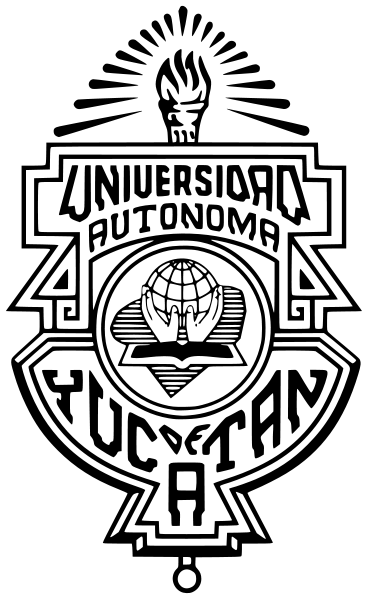
\includegraphics[scale=0.3]{UADY.png}
	\end{figure}}
	\vspace{0.7cm}
	{\Large\itshape Erick Al. Casanova Cortés\par}
	{\Large\itshape Matricula: 15014866\par}
	\vfill
	{\scshape\Large Docente\par
	Dr. German Giacoman\par}
	\vfill
	{\Large{\bfseries Fecha de modificación: \today} }

	\vfill
	
\end{titlepage}

%-------------------------------------------------
%Inicio del documento
%-------------------------------------------------
\tableofcontents

%-------------------------------------------------
%Fundamentos de termoquímica
%------------------------------------------------

\chaper{Fundamentos de termoquímica}


La fisicoquímica es la parte de la Química que estudia las propiedades físicas y la estructura de la materia, las leyes de las interacciones química sy las teorías que las gobiernan, La fisicoquímica se encarga de recabar los datos necesarios que permitan establecer las propiedades que presenten la materia a fin de sistematizarlo a través de leyes y darles un formato teórico.

\subsection{deferencias entre el enfoque cinético y térmico}
Ambos enfoques se aplican a los fluidos para estudiar sus propiedades y los fenómenos en los que participan

El enfoque \textbf{termodinámico} se basa en observaciones de cambios de energía que se da entre la etapa inicial y final del proceso

El enfoque \textbf{cinético} Intenta describir a detalle los pasos que se desarrollan en los cambios que se producen durante la transformación de la materia en un proceso dado



%-------------------------------------------------
%Equilibrio químico
%------------------------------------------------


\chaper{Equilibrio químico}

%-------------------------------------------------
%Cinetica química y catálisis
%------------------------------------------------

\chaper{Cinetica química y catálisis}

%-------------------------------------------------
%Fotoquímica
%-----------------------------------------------

\chaper{Fotoquímica}

%-------------------------------------------------
%Fenómenos superficiales y sistemas coloidales
%------------------------------------------------

\chaper{Fenómenos superficiales y sistemas coloidales}


%-------------------------------------------------
%Final del documento
%-------------------------------------------------

\end{document}
